\chapter{Model and methods}
\label{chap:modmet}
\section{Description of the WRF-ARW Modeling System}
\label{sec:modeldes}
%(What did Johanne and Kjetil and Linda Bjørn Egil think was important enough to write about in their thesees?)
To produce results for the thesis, a formulation of the Weather Research and Forecasting (WRF) Model called the Advanced Research WRF (ARW) has been used, Version 3.6.1, released in April 2014. The model is primarily developed at the National Centre for Atmospheric Research (NCAR) in Boulder, Colorado. The ARW model is the first fully compressible conservative form nonhydrostatic model designed for both research and operational numerical weather prediction (NWP) applications~\citep{Skamarock2008}. 

As can be seen from figure~\ref{fig:wrfflowchart} the WRF-ARW Modeling System consists of four major programs~\citep{Wang2015}:
\begin{itemize}
\item The WRF Prepocessing System (WPS)
\item WRF-Data Assimilation (WRF-DA)
\item ARW solver
\item Post-processing \& Visualization tools
\end{itemize}

WPS is used primarily for real data simulations~\citep{Wang2015}, like the study presented in this thesis. Its functions include defining simulation domains, interpolating terrestrial data and degribbing and interpolating meteorological data from another model to this simulation domain~\citep{Wang2015}. WRF-DA is optional and can be used to ingest observations into the interpolated analyses created by WPS~\citep{Wang2015}, but was not used in this study. The ARW solver is the key component of the modeling system, which is composed of several intialization programs for idealized, and real-data simulations, and the numerical integration program~\citep{Wang2015}. Fully compressible nonhydrostatic equations with hydrostatic options, regional and global applications, complete coriolis and curvature terms and that vertical grid-spacing can vary with height are among the WRF models key features according to~\citet{Wang2015}.

\begin{figure}
\centering
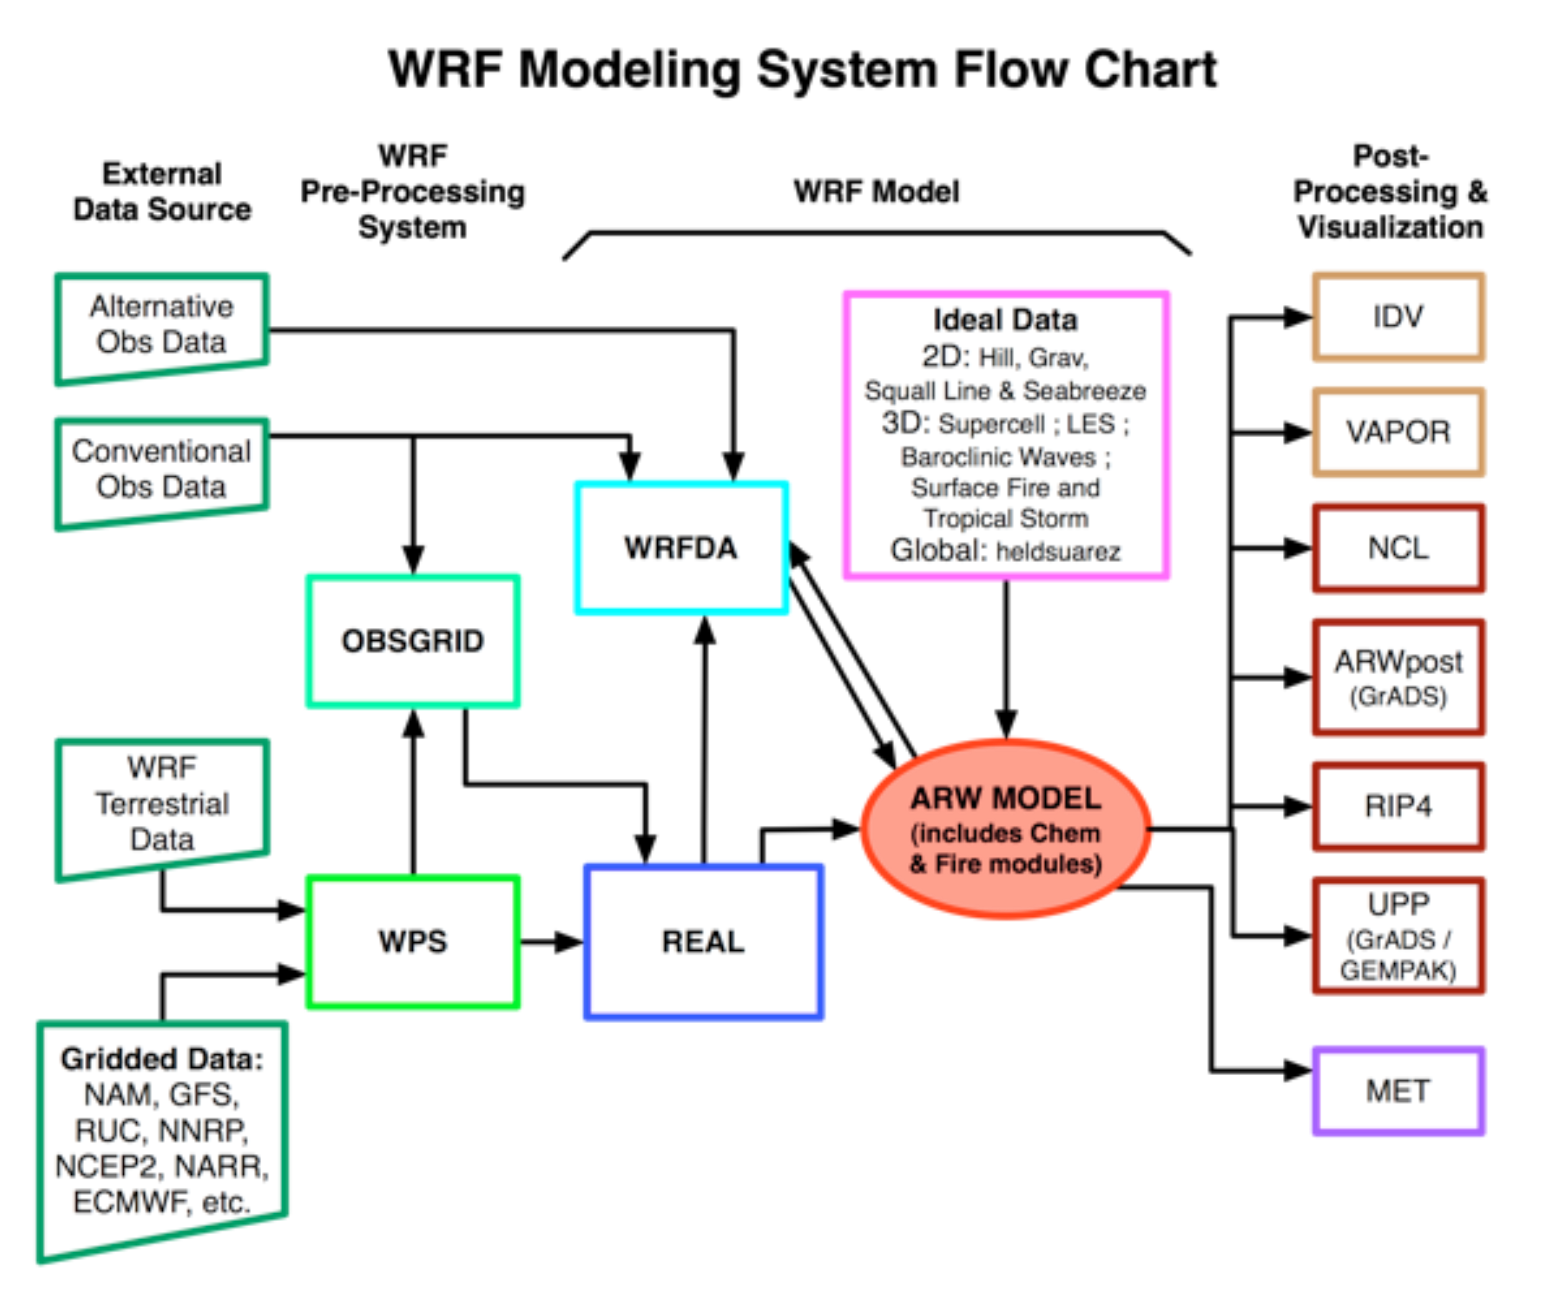
\includegraphics[width=\textwidth]{model_methods/wrfflowchart}
\caption{Flowchart for the WRF ARW Modeling System Version 3. From~\citet{Wang2015}.}
\label{fig:wrfflowchart}
\end{figure}

The model can be run for ideal cases or real-data cases. I have run the real-time WRF, real.exe — to produce inputfiles for the ARW solver, wrf.exe.
%Any detailed information on the model, presented in this section is based on the Article by~\citet{Skamarock2008} unless otherwise stated.

The continuous equations solved in the ARW model are the Euler equations cast in a flux form where the vertical coordinate, $\eta$, is defined by a normalized hydrostatic pressure,
\begin{equation}
\eta = (p_h - p_{ht})/\mu 
\end{equation}
where $\mu = (p_{hs} - p_{ht})$~\citep{Skamarock2008}. $p_h$ is the hydrostatic component of the pressure and $p_{hs}$ and $p_{ht}$ are the values of the hydrostatic pressure in a dry atmosphere at the surface and top boundaries respectively~\citep{Skamarock2008}.

The vertical coordinate is the traditional $\sigma$ coordinate used in many hydrostatic atmospheric models, shown in a diagram in figure~\ref{fig:sigma}.

\begin{figure}
\centering
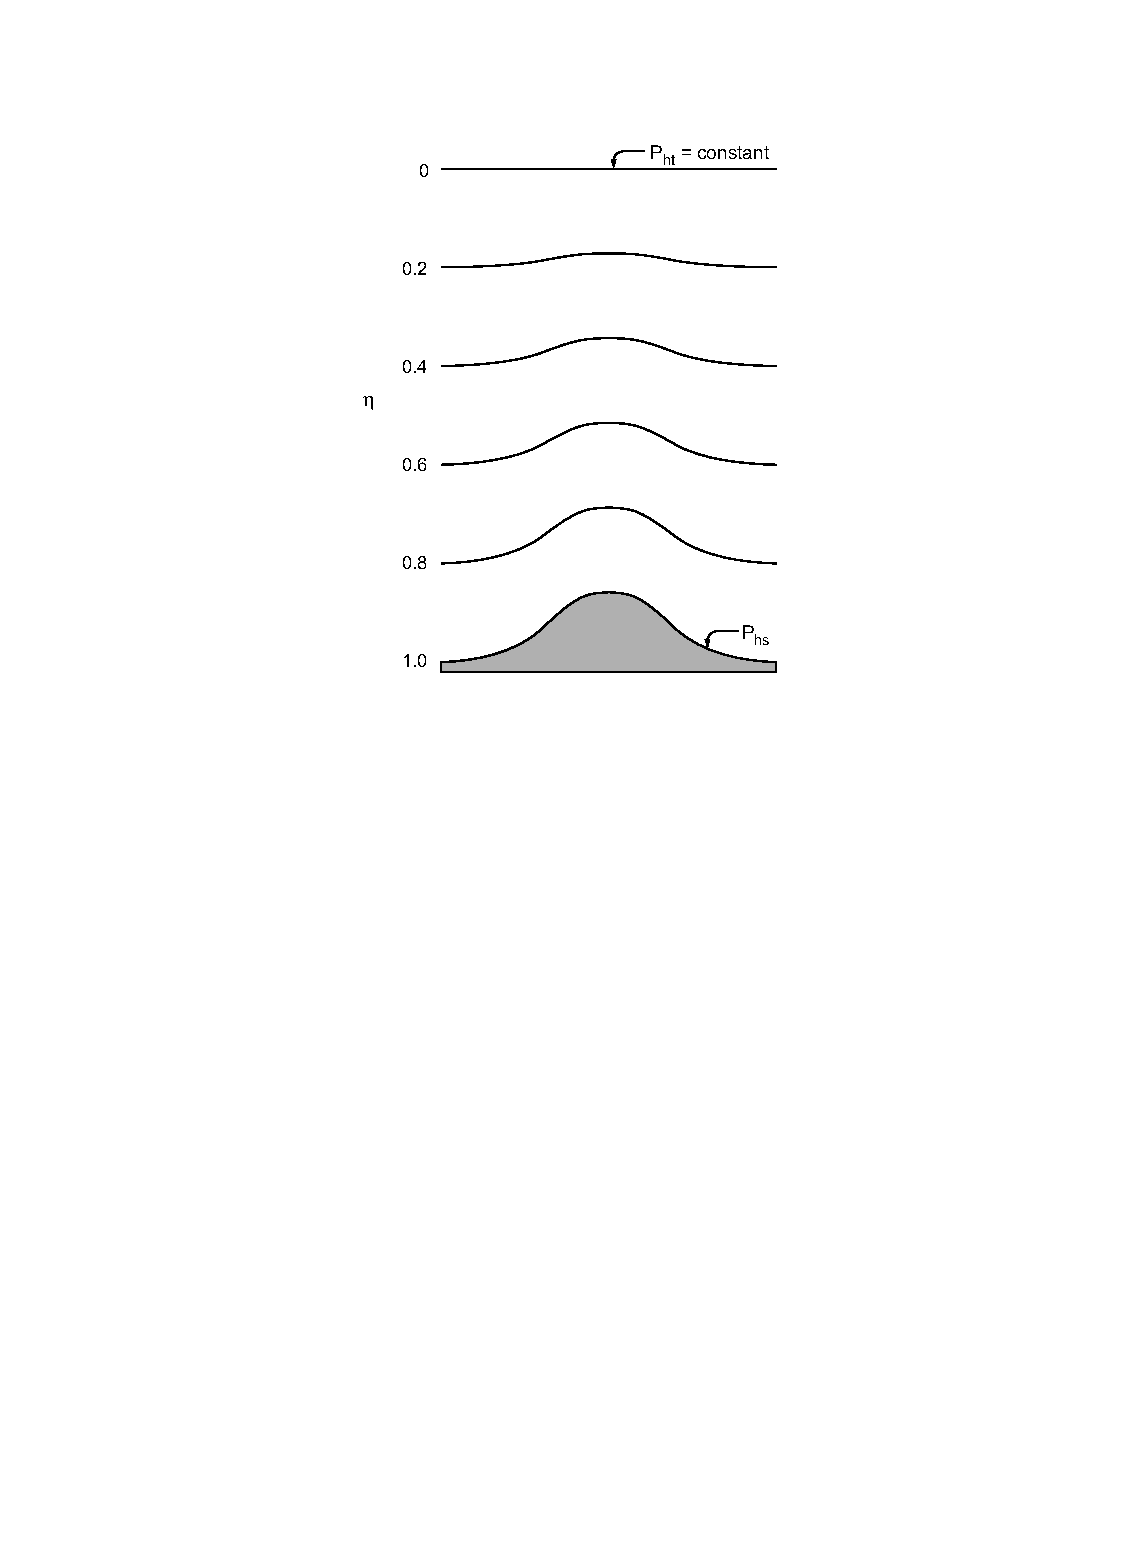
\includegraphics[scale=1]{model_methods/sigma.pdf}
\caption{This figure is shown as presented in~\citet{Skamarock2008}, and is a schematic of the terrain following a $\sigma$ coordinate. $P_{hs}$ and $P_{ht}$ is the hydrostatic pressure at the surface and the top respectively.}
\label{fig:sigma}
\end{figure}

\subsection{Physics, radiation and interactions in WRF}
Based on the WRF-ARW Version 3 User's Guide by~\citet{Wang2015}.
%Based on the description of ARW Version 3 from \citet{Skamarock2008a}. 
The physics options in WRF fall into several categories, each containing several choices. Table~\ref{tab:physics} shows som of the different categories and the choice of scheme within each category.

\begin{table}[H]
\centering
\caption{Table of physics categories and choice of scheme for this thesis}
\label{tab:physics} 
\begin{tabular}{L{6.cm} L{6.cm}}
\centering
\textbf{Physics categories} & \textbf{Scheme selected within category}\\ \hline
(1) microphysics & aerorol-aware ~\citep{Reisner1998, Thompson2004, Thompson2008, Thompson2014}. Option 28.\\
(2) cumulus parameterization & Grell 3D  @cite authors. Option 5.\\
(3) planetary boundary layer (PBL) &  Yonsei University scheme @cite authors. Option 1.\\
(4) land-surface model & Noah Land Surface Model @cite authors. Option 2.\\
(5) radiation & RRTMG LW \& SW ~\citep{Mlawer1997, Iacono2000, Iacono2003, Iacono2008}. Radiation options 4.\\
\end{tabular}
\end{table}

The microphysics includes explicitly resolved water vapor, cloud, and precipitation processes. The aerosol-aware scheme was chosen to have scavenging of aerosols and have proper enough representation of aerosols to study aerosol-cloud interactions, without using the WRF model coupled with chemistry (WRF-Chem).

The choice of cumulus parameterization was based on the grid resolution, and the best fit for it. A horisontal grid spacing of 4~km can be fine enough to not use cumulus parameterization, but in this thesis I chose a parameterization that was more suitable for grid sizes less than 10~km, the Grell 3D parameterization. Grell 3D is an improved multi-closure, multi-parameter ensamble method with typically 144 sub-grid members, that may be used on high resolution~\citep{Wang2015}, like my 4~km grid spacing.

Yonsei University scheme was chosen for the PBL. It is a non-local-K scheme with explicit entrainment layer and parabolic profile in unstable mixed layer~\citep{Wang2015}.

The land-surface model choice came to Noah Land Surface Model. The Noah Land Surface Model, is a unified NCEP/NCAR/AFWA (National Centers for Environmental Prediction, National Centre for Atmospheric Research, Air Force Weather Agency) scheme with soil temperature and moisture in four layers which provides sensible and latent heat fluxes to the PBL scheme~\citep{Wang2015}. Additionally, it predicts soil ice, and fractional snow cover effects, which could be important in the Arctic, but it is probably not the most important choice, since there is very little land in the area investigated, see figure~\ref{fig:area} in Chapter~\ref{chap:introduction}.

The radiation schemes were chosen simply because they are the best match for the microphysics scheme at the time of writing. According to~\citet{Thompson2014} the Rapid Radiative Transfer Model (RRTM) for General Circulation Models (GCMs) (RRTMG) schemes for SW and LW are the only radiation schemes which include the effects of the effective radii calculated in aerosol-aware. The RRTMG schemes are accurate schemes using look-up tables for efficiency, and accounts for multiple bands and microphysics species, and includes the Monte Carlo Independent Column Approximation (MCICA) method of random cloud overlap~\citep{Wang2015}. Major trace gases are constant in my runs, and their values are $CO_2=379e-6$, $N_2O=319e-9$, $CH_4=1774e-9$~\citep{Wang2015}.

\section{Schemes}
\label{sec:schemes}
The ARW model offers a wide selection of schemes to treat different physics that one wants represented in the model. The schemes treat the physics slightly differently and some schemes are better for certain horisontal and vertical resolutions than others, so one needs to be careful when choosing how the model is to treat the physics. For my thesis, the especially relevant scheme to mention is the cloud microphysics scheme that I chose, which is the aerosol-aware scheme described in~\citet{Thompson2014} which is a development of the bulk microphysisc scheme described in~\citet{Thompson2008}, to include aerosols and scavenging of them. The scheme is a true double moment scheme and therefore treats cloud water, cloud ice, rain and snow in a complex and detailed way~\citep{Thompson2014}. At the time of writing, the only radiation schemes that make use of the effective radii are the RRTMG radiation schemes~\citep{Mlawer1997, Iacono2000, Iacono2003, Iacono2008} for both SW and LW. These were therefore used in combination with the aerosol-aware cloud microphysics scheme.

\subsection{The aerosol-aware scheme}
According to the ARW User's Guide by~\citet{Wang2015}, the aerosol-aware scheme considers water- and ice-friendly aerosols, and a climatological dataset may be used to specify initial and boundary conditions for the aerosol variables. I have used this climatological dataset, which is explained in Section~\ref{sec:inputdata}~Input~data. The scheme uses a monthly mean for aerosol number concentrations derived from multi-year (2001-2007) global model simulations %@citationColarco2010??(det har de cita)
in which particles and their precursors are emitted by natural and anthropogenic sources and are explicitly modeled with multiple size bins for multiple species of aerosols by the Goddard Chemistry Aerosol Radiation and Transport (GOCART) model %(@desiterteGinoux2001)
~\citep{Thompson2014}.
The microphysics option 28, the aerosol-aware scheme~\citep{Thompson2014} is built on the schematic shown in figure~\ref{fig:microphysics}, from~\citet{Reisner1998}. It is a double moment scheme, which means it computes both mass mixing ratios, Q, and number concentrations, N, for the same water species (hydrometeors). 

\begin{figure}
\centering
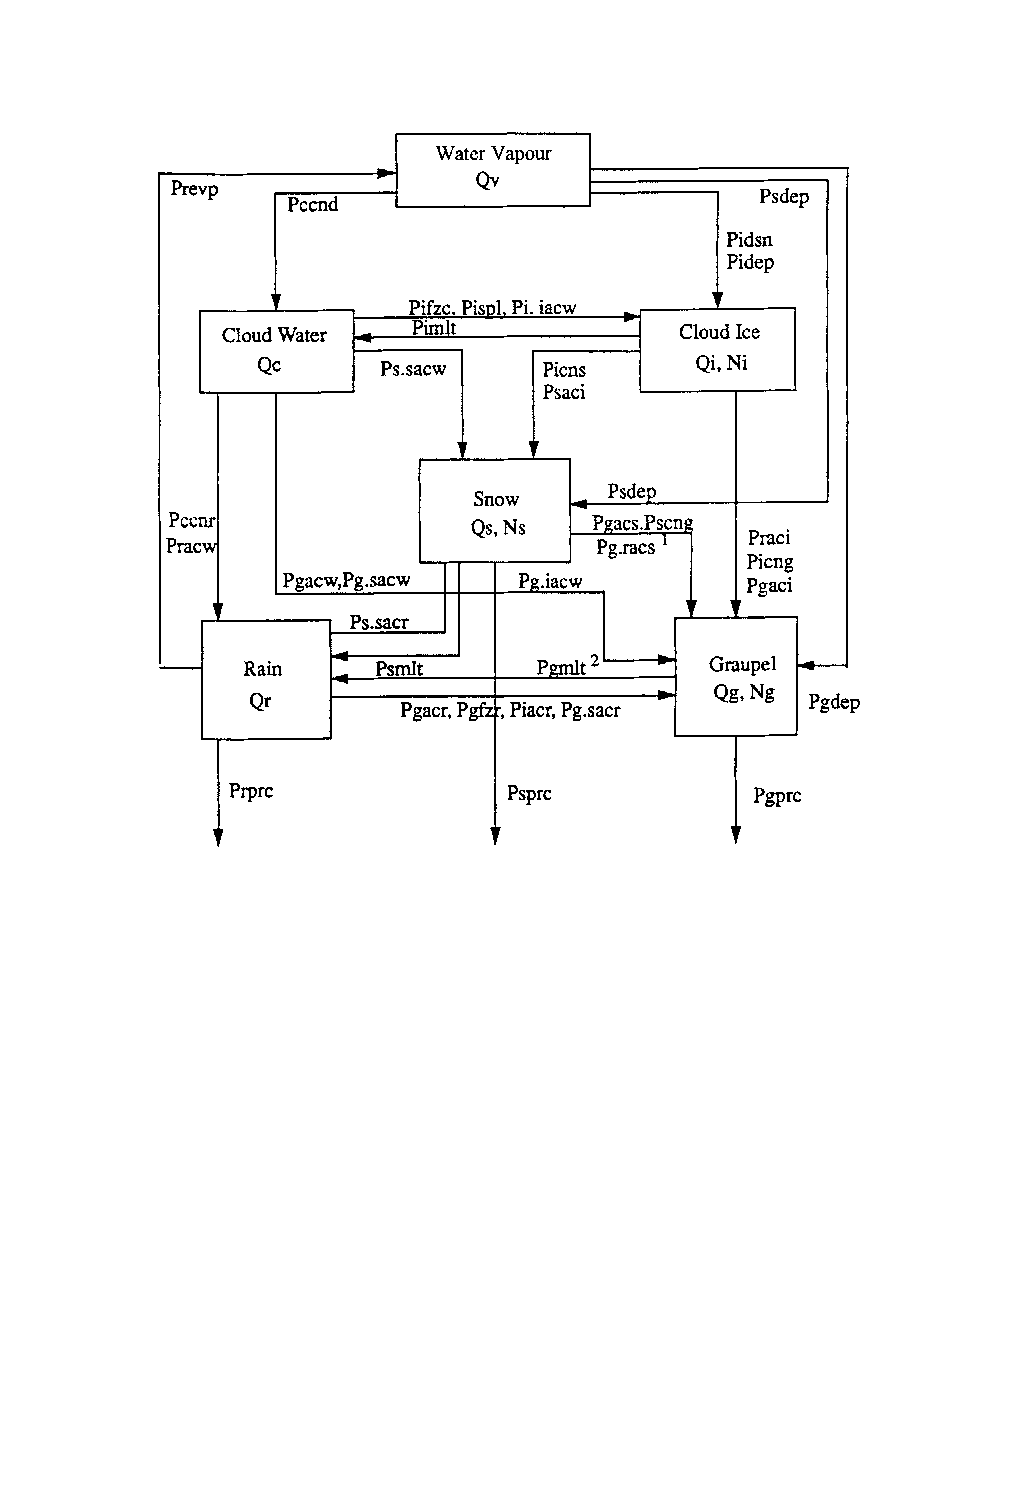
\includegraphics[scale=0.8]{model_methods/microphysics.pdf}
\caption{Cloud microphysical parameterization scheme typically used i NWP models as shown in~\citet{Reisner1998}. A full list of the acronyms used in the schematic can be found in~\citet{Reisner1998}.}
\label{fig:microphysics}
\end{figure}

Figure~\ref{fig:microphysics} show the processes in the microphysics scheme developed by~\citet{Reisner1998}, which the first bulk microphysics scheme by Thompson~\citep{Thompson2004} was based on. The aerosol-aware scheme~\citep{Thompson2014} is an extension of the updated Thompson bulk microphysics scheme described in~\citet{Thompson2008}. The figure shows a schematic of five hydrometeors, cloud water (c), rain (r), ice (i), snow (s) and graupel (g), and if just the mass mixing ratio is calculated or if both the mass mixing ratio and the number concentration is calculated. For each of the hydrometeors, prognostic equations are used with all the sources and sink terms included.%, as exemplified by this equation from~\citet{Reisner1998}
%\begin{equation}
%
%\end{equation}
 % which was originally built on this~\citep{Thompson2004}, but there is not much left of it in the code now (@cite the code comments?).

\subsection{The RRTMG radiation schemes}
The RRTM scheme described in~\citet{Mlawer1997} uses the correlated-k method, which is an appriximated technique for the accelerated calculation of fluxes and cooling rates for inhomogeneous atmospheres~\citep{Mlawer1997}. %\textbf{@define inhomogeneous atmosphere}.
The correlated-k method is capable of achieving accuracy comparable with that of line-by-line models with an extreme reduction in the number of radiative transfer operations performed~\citep{Mlawer1997}, which by that reduces computational cost and increases computational efficiency. The Line-By-Line Radiative Transfer Model (LBLRTM) is used both to calculate the absorption coefficients used to generate the k distributions needed by RRTM and  to evaluate the RRTM calculations of fluxes and cooling rates~\citep{Iacono2000}. 


\section{Model setup}
\label{sec:modelsetup}
The covers parts of the Beaufort Sea and the East Siberian Sea, by Canada and Alaska. This area was chosen because data from the area has been used for related studies~\citep{Intrieri2002,Shupe2004,Kay2009,Wu2012,Palm2010,Schweiger2008} %sjekk dette!!,
which were mentioned in Chapter~\ref{chap:background}~Background.%, to give the reader some background material and an understanding of the subject of this study.
The area is not completely ice free any part of the year,% @cite,
 and provides a good place to simulate cloud and sea ice interaction. The area is over several time zones but is approximately 7 hours behind UTC time. The times given in the WRF-ARW modeling system are UTC. This means that figures showing 1200 UTC are for approximately 0500 h local time in Canada and Alaska.

I ran ARW with a horisontal resolution of 4~km spacing between the grid points, and a vertical resolution of 72 vertical layers from the surface to the model top at 10hPa. This resolution is sufficient to resolve clouds.% @citation. 300~$\cdot$~300 gridpoints, with 4~km spacing, between .
The vertical layers in the ARW model are often referred to as eta levels, because of the choice of $\eta$ as the vertical coordinate. These levels have uneven vertical spacing. The fact that this $\eta$ is the traditional $\sigma$-coordinate, means that the altitude of each level is dependent on pressure, therefore the level height varies in both time and space. As a consequence of pressure dependence, the levels in the lower troposphere are closer to each other than the levels higher up in the troposphere. Therefore the low clouds in the area can be resolved. Approximate heights for the lowest 11 eta levels is shown in Table~\ref{tab:etaheights}.

\begin{table}[H]
\centering
\caption{Approximate height for each level in meters above the sea surface for the part of the level that is over the sea, and meters above topography for the part of the level that is over land.}
\label{tab:etaheights} 
\begin{tabular}{C{6.cm} C{6.cm}}
\centering
\textbf{Eta level} & \textbf{Approximate height}\\ \hline
1 & 10~m\\
2 & 50~m\\
3 & 130~m\\
4 & 230~m\\
5 & 370~m\\
6 & 530~m\\
7 & 650~m\\
8 & 950~m\\
9 & 1250~m\\
10 & 1400~m\\
11 & 1600~m
\end{tabular}
\end{table}

The sea ice in the area was removed, by editing the input file made by WPS and real.exe, to get results to compare with results from runs with ice.

From diminishing sea ice we might experience an increase in sea traffic, which would lead to an increase in aerosol content in otherwise clean air.% @citation.
To include increase in aerosol concentrations due to lack of sea ice I used the microphysics scheme developed by Greg Thompson and Trude Eidhammer described in~\citet{Thompson2014}.

%Choice of schemes and reasons should be presented. As should how WPS and real.exe and wrf.exe works. At least short about what they do and contribute with to get to the end results. Explain some of the improvements in the micro physics scheme in combination with the revised radiation schemes (RRTMG for SW and LW).

\section{Model runs}
\begin{table}[H]
\centering
\caption{Table showing the name of the runs and what is included}
\label{tab:runs} 
\begin{tabular}{L{2.3cm} L{2.3cm} L{2cm} L{1.5cm} L{1cm} L{1cm} L{3cm}}
\centering
Name & Horisontal resolution & Dimensions & Vertical layers & $\Delta$t & Sea ice & Aerosol concentration\\ \hline
control & 4~km x 4~km & 300 x 300 & 72& 24~s & yes & control\\
NoIce & 4~km x 4~km & 300 x 300 & 72 & 24~s & no & control\\
Aero10 & 4~km x 4~km & 300 x 300 & 72 & 24~s & yes & control x 10\\
Aero10NoIce & 4~km x 4~km & 300 x 300 & 72 & 24~s & no & control x 10\\
Aero100 & 4~km x 4~km & 300 x 300 & 72 & 24~s & yes & control x 100\\
Aero100NoIce & 4~km x 4~km & 300 x 300 & 72 & 24~s & no & control x 100 \\
\end{tabular}
\end{table}

Which table?

\begin{table}[H]
\centering
\caption{Caption could say: Table showing the names of the runs and if they have sea ice or not, and if the aerosol concentration has been increased by a factor of 10 or 100 through input files. All the runs have the same horisontal resolution of 4kmx4km, dimensons 300x300, vertical layers 72 and time step 24 s.}
\label{tab:runs} 
\begin{tabular}{L{2.3cm} L{2cm} L{3cm}}
\centering
Name & Sea ice & Aerosol concentration\\ \hline
control & initial & control \\
NoIce & removed & control \\
Aero10 & initial & control x 10 \\
Aero10NoIce & removed & control x 10 \\
Aero100 & initial & control x 100 \\
Aero100NoIce & removed & control x 100 \\
\end{tabular}
\end{table}

\subsection{Manipulation of input files}
wrfinput\_d01 and wrfbdy\_d01 are input files for domain 1, in my case the only domain, and are made by real.exe. These files are then used as initialization or forcing when wrf.exe is run.
To run the model without ice and with an increased number of aerosols I manipulated the input files for WRF. I used a netCDF Operator (NCO) tool, ncap2. This allowed me to manipulate the netCDF files from my terminal window in the folder where they were located.
Elaborate on removal or placing of sea ice. Elaborate on multiplying the aerosol number concentration with a factor 10 or 100. By use of ncap2 from NetCDF (NCO).

\subsection{Changed ice run}
The sea ice was removed. 
The point of this is to compare the run with no ice to the control run, and see if there are any changes to the cloud properties.

\subsection{Changed aerosols run}
The increase in aerosol concentration was a bit more complicated, but the same method. The number of water and ice friendly aerosols were multiplied by 100 and so were their tendencies and respective concentrations at the boundaries of the area. The goal is to find changes in cloud properties compared to those in the control run, for that purpose the aerosol concentration was multiplied by a factor of 10 and another by a factor of 100. Hoping to get a signal.

\section{Input data}
\label{sec:inputdata}
The model runs were initialized with data downloaded from the European Centre for Medium-Range Weather Forecasts (ECMWF)~@cite web page.%was downloaded from their site and used as input for initial and boundary?? conditions.
The downloaded data is from the ERA-Interim dataset, which is a global atmospheric reanalysis from 1979 to present and continues to be updated in real time.%~\citet{ecmwf}.@make bib for ecmwf
Through WPS the data from ERA-Interim was interpolated over the area, with a 2 degree minute spacing between the points, to be used to initialize the model. The data used is in 6-hourly atmospheric fields on pressure levels, for the first five days of September 2012, which was the period the model was run for. This is done to make sure the initial meteorological conditions are the same in every run, so that the effects of changing a variable in the input files for the modeling system are only due to that change.

%Explain the use of climatological data for aerosol input.
To use the climatological aerosol dataset, the file containing monthly means had to be called through WPS for real.exe to make input data for water- and ice-friendly aerosols in the wrfinput\_d01 and wrfbdy\_01 files. The aerosol input data includes mass mixing ratios of sulfates, sea salts, organic carbon, dust, and black carbon from a 7-yr simulation with 0.5$^{\text{o}}$ longitude by 1.25$^{\text{o}}$ latitude spacing~\citep{Thompson2014}.

\section{Processing of the results}
Figures presented in my thesis, I made (unless other is stated) by use of National Centre for Atmospheric Research (NCAR) Command Language (NCL) and MatLab. For the NCL scripts I found a lot of help and inspiration from the example scripts for WRF-users available at (URL for examples).

I made all the figures that are over maps with NCL, the others were made with MatLab provided by the University of Oslo.

%MathWorks, it is very useful and easy to use.

%NCL it is free and there are a lot of available example scripts to quickly learn how to use the graphics.